\lecdate{20.03.2017}
\slides[0.5]{STTI_intro_2017}{6}
% Passwort: Tallinn11
\section{Einführung}
\subsection*{Ziel der Vorlesung}
\slides{reliability/contents}{2}
\subsection{Zuverlässige / fehlertolerante Systeme}
\slides{reliability/contents}{4}
Einfachstes Mittel für besser Reliability: \emph{Redundanz}\\
Failur classes … meint Fehler-Klassen von kritischen Fehlern (Versagen)
\subsection{Modellierung fehlertoleranter Systeme}
\slides{reliability/contents}{5}

\section{Grundlegende Zuverlässigkeitsquantifizierung}
\slides{reliability/contents}{3}
Reliability … Zuverlässigkeit / Wahrscheinlichkeit, dass ein System über eine Zeit funktionsfähig ist\\
Availability … Verfügbarkeit (pro Zeit)\\
Mission time … Wie lange soll ein System ohne Reparatur „im Feld“ bleiben?

\subsection{Wie lang läuft ein System ohne Versagen?}
\slides{reliability/part1}{3}
\slides{reliability/part1}{4}
Also: Der Mittelwert gibt keine Garantie, dass das Gerät bis zu einer bestimmten Zeit läuft.

\subsection{Wie Wahrscheinlich ist die fehlerfreie Nutzung für einen bestimmten Zeitraum?}
\slides{reliability/part1}{5}
\slides{reliability/part1}{6}

\subsection{Versagenswahrscheinlichkeit und Zuverlässigkeit}
\slides{reliability/part1}{7}
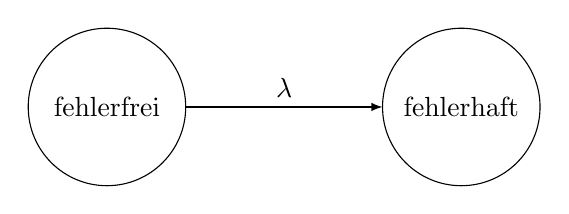
\begin{tikzpicture}
\draw  (-4.5,0) node{fehlerfrei} circle (1);
\draw  (0,0)  node{fehlerhaft} circle (1);
\draw[-latex] (-3.5,0) -- (-1,0) node[pos=.5, above]{$\lambda$};
\end{tikzpicture}\\
$R(t)=P(fehlerfrei)$\\
$R(t)=e^{-\lambda t}$\\
$R'(t)=-\lambda R(t)$

\subsection{Mittlere Zeit bis zum Versagen (MTTF)}
\slides{reliability/part1}{8}
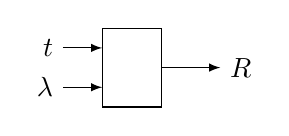
\begin{tikzpicture}[scale=.5]
\draw  (-1.5,2) rectangle (0,0);
\draw [-latex] (-2.5,1.5) node[left]{$t$} -- (-1.5,1.5);
\draw [latex-] (-1.5,0.5) -- (-2.5,0.5) node[left]{$\lambda$};
\draw [-latex] (0,1) -- (1.5,1) node[right]{$R$};
\end{tikzpicture}\\
$MTTF=P(L>t)=E(t)=\frac{1}{\lambda}$\\
Bspw.: $\lambda=5 \frac{1}{year} \to MTTF=\frac{1}{5}year$

\subsection{Verfügbarkeit}
\slides{reliability/part1}{9}
\slides{reliability/part1}{10}

\subsection{Beispiel Versagen und Verfügbarkeit}
\subsubsection{Einzelne Komponente ohne Reparatur}
\slides{reliability/part1}{11}
Die Einsatzdauer sollte immer deutlich kürzer sein, als die MTTF (da $R(MTTF)=0,37$ -- also die Fehlerrate zur mittleren Versagenszeit -- ein sehr schlechter Wert ist).
\subsubsection{Einzelne Komponente mit Reparatur}
\slides{reliability/part1}{12}

\subsection{Systemstruktur}
\slides{reliability/part1}{13}
\subsubsection{Zusammensetzung in Reihe}
\lecdate{27.03.2017}
\slides{reliability/part1}{14}
\slides{reliability/part1}{15}
\subsubsection*{Verfügbarkeit}
\slides{reliability/part1}{16}
\subsubsection{Parallele Zusammensetzung}
\slides{reliability/part1}{17}
\slides{reliability/part1}{18}

\subsection{Zusammenfassung}
\slides{reliability/part1}{20}
\slides{reliability/part1}{21}

Beispiele für Systeme, die zuverlässig sein müssen: Flugzeug(-klappensteuerung), Atomkraftwerksteuerung, medizinische Geräte, Rechenzentren, …

\section{Zuverlässige/Fehlertolerante Systeme}
\slides{reliability/part2}{2}
\subsection{Verlässliches System}
\slides{reliability/part2}{3}
\slides{reliability/part2}{4}
\subsection{Fehlertolerantens System}
\slides{reliability/part2}{5}
\slides{reliability/part2}{6}
\subsection{Fehlerklassen}
\slides{reliability/part2}{7}
(von unten noch oben immer allgemeinere Fehler)
\slides{reliability/part2}{8}
\subsection{Techniken zur Fehlertoleranz}
\subsubsection{Redundanz}
\slides{reliability/part2}{9}
\slides{reliability/part2}{10}
\slides{reliability/part2}{11}
\subsubsection{Fehlerisolation, Wiederherstellung und Fehlerkompensation}
\slides{reliability/part2}{12}
\subsubsection{Rekonfigurierung (DMR, PSR, TMPR)}
\slides{reliability/part2}{13}
\subsubsection*{DMR System}
\slides{reliability/part2}{14}
\subsubsection*{PSR System}
\slides{reliability/part2}{15}
\subsubsection*{TMPR System}
\slides{reliability/part2}{16}
\subsubsection*{Replikation mit verteilter Mehrheitswahl}
\slides{reliability/part2}{17}

\subsection{Systemschichten und Fehlertoleranztechniken}
\slides{reliability/part2}{19}
\slides{reliability/part2}{20}
\slides{reliability/part2}{21}

\subsection{Grundlegende Techniken der Fehlertoleranz}
\slides{reliability/part2}{22}
\subsubsection*{Beispiele}
\slides{reliability/part2}{23}
\slides{reliability/part2}{24}

\subsection{Zusammenfassung}
\slides{reliability/part2}{25}


\section{Zuverlässigkeitsmodellierung}
\slides{reliability/part3}{2}
\subsection{Systemstruktur}
\slides{reliability/part3}{3}
\subsection{Boolsche Modelle}
\slides{reliability/part3}{4}
\subsection{Veranschaulichung Boolscher Modelle}
\slides{reliability/part3}{5}
\subsubsection{Fehlerbäume}
\slides{reliability/part3}{6}
\subsubsection*{Beispiele}
\slides{reliability/part3}{7}
\slides{reliability/part3}{8}
\subsubsection{RBD (Reliability Block Diagramm)}
\slides{reliability/part3}{9}
\subsection{Arbeiten mit Wahrscheinlichkeiten}
\slides{reliability/part3}{10}
\subsubsection{(k von k+m)-System}
\slides{reliability/part3}{11}
\subsubsection*{Beispiele}
\slides{reliability/part3}{12}
\slides{reliability/part3}{13}

\subsubsection{R und F als Funktionen der Zeit}
\slides{reliability/part3}{14}
\slides{reliability/part3}{15}

\subsection{Zussamenfassung: Statische Systemkonfigurierung}
\slides{reliability/part3}{16}

\subsection{Dynamische fehlertolerante Systeme mit Reparatur}
\slides{reliability/part3}{17}
\subsection{Markov Modelle}
\slides{reliability/part3}{21}
\slides{reliability/part3}{22}
\subsubsection{Einzelne Komponente ohne Reparatur}
\slides{reliability/part3}{23}
\subsubsection{Einzelne Komponente mit Reparatur}
\slides{reliability/part3}{24}
\subsubsection{Allgemeines Markov Modell eines Zweikomponentensystems}
\slides{reliability/part3}{25}
\subsubsection*{1 von 2 System mit Reparatur}
\slides{reliability/part3}{26}
\subsubsection{Allgemeines Markov Modell eines Dreikomponentensystems}
\slides{reliability/part3}{27}
\subsubsection*{3 von 2 System ohne Reparatur}
\slides{reliability/part3}{28}
\subsubsection*{2 von 3 System mit Reperatur}
\slides{reliability/part3}{29}
\subsubsection{Markovketten Simulator}
\slides{reliability/part3}{30}
\subsection{Zusammenfassung}
\slides{reliability/part3}{31}
\slides{reliability/part3}{32}












